\documentclass{article}
% set up the page formatting
\usepackage[a4paper, portrait, margin=2.5cm]{geometry}
\usepackage{multicol}
\usepackage{fancyhdr}
\usepackage{graphicx}
\usepackage{float}

% allow for table of contents to have clickable links
\usepackage{hyperref}

% editable bits
\title{CS261 Group 29 Requirement Analysis}
\author{Ani Bitri, Krister Hughes, Thomas Phuong, Eshan Sharif, Josh Turner, Antoni Zyla}
\date{January 2025}
\fancyfoot[L]{Requirement Analysis}
\fancyfoot[R]{\thepage}

\begin{document}
\maketitle

% table of contents would exceed the page limit
% \tableoddfcontents

\section{Introduction}
% Justifies the need for the system and outlines what it will do.
Dorset Software has been contracted to create a system used for the modelling 
of traffic junctions based on various parameters. The system will provide 
data about how each of these configurations impacts the performance of a given 
junction and allow for the comparison of various sets of parameters to help 
determine the best configuration for a given junction. As a group, we have been 
given the task of developing this system, along with managing the project and 
creating documentation.

\section{System Architecture}
% Presents a high-level overview of the system, showing distribution of functions across system modules.
% Make sure that the requirements are in order of priority
\begin{figure}[H]
    \centering
    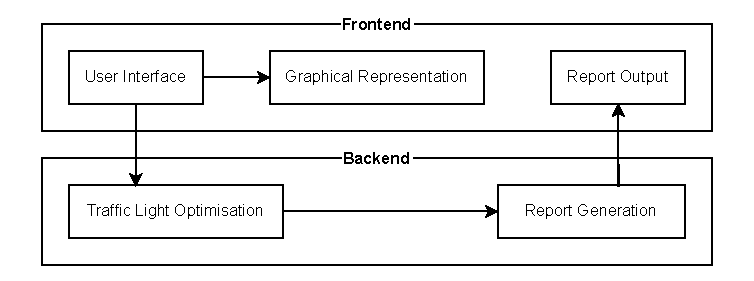
\includegraphics[width=0.5\linewidth]{System architecture.drawio.pdf}
    \caption{System Architecture Diagram}
    \label{system architecture}
\end{figure}
A high-level overview of how we intend the system to work is as follows: the user will 
enter the traffic flow rates for the simulation and select the configurable parameters 
for each junction configuration via the user interface, leading to the graphical 
representation displayed updating to reflect the user input. After pressing a button to 
start the simulation, the user input will be sent to the backend, where each junction 
configuration will be simulated and have its traffic light sequencing optimised based on 
the parameters restricting the order and the best values of the junction efficiency metrics. 
After all junction configurations have been processed, the data will be sent back to the 
frontend to generate a report of the efficiency of each junction configuration.

\section{System Requirements Specification}
% Describes functional and non-functional requirements.
\subsection{Functional Requirements}
\begin{itemize}
    \item \textbf{\underline{Requirement 1 (Must)}}
    \begin{itemize}
        \item \textbf{C}: The user must be able to input the rate of traffic flow from 
            each direction to each other direction via text fields (one per traffic flow) 
            in the User Interface (UI).
        \item \textbf{D}: The system must accept input from the text fields, parse the input to 
            determine if each traffic flow is a valid number, and, if all traffic flows 
            are valid, allow the simulation to be run.
        \item \textbf{Verification}: running the simulation with one set of valid traffic 
            flow rates in the text fields, running it again with a different set in 
            the same fields and verifying the junction efficiency metrics have changed, 
            and then trying to run the simulation with an invalid value in at least one 
            text field (e.g. “TEST” for Eastbound Traffic Flow Exiting West)
        \item\textbf{Traceability}: Input Parameters section in the specification
    \end{itemize}
    
    \item \textbf{\underline{Requirement 2 (Must)}}
    \begin{itemize}
        \item \textbf{C}: The user will be able to adjust the number of lanes (between 1 and 5) 
            and toggle left lanes, right lanes, bus lanes, and pedestrian crossings. They will 
            also be able to configure the timings and frequency of pedestrians crossing.
        \item \textbf{D}: For a given configuration the system will determine if it is a valid 
            configuration.
        \item \textbf{Verification}: run a simulation with default parameters (2 lanes per 
            road entering the junction, equal priority on all lights, and all other 
            settings set to off/No) as a reference, and then run a simulation per setting 
            with that setting adjusted, showing the results of each simulation is different 
            from the reference.
        \item\textbf{Traceability}: Configurable Parameters section in the specification well
    \end{itemize}

    % Insert requirement for priority

    \item \textbf{\underline{Requirement 3 (Should)}}
    \begin{itemize}
        \item \textbf{C}: The user will be presented with a graphical representation of the junction 
        based on the parameters they have entered.
        \item \textbf{D}: The system must take the current configuration settings of the junction and 
        generate a representation of the junction which mirrors those settings. 
        \item \textbf{Verification}: Junctions can be generated with all lane counts from 1-5, then 
        with a left and right lane, a pedestrian crossing, and a bus lane. We will also check that 
        lanes display correctly in each orientation.
        \item\textbf{Traceability}: Output section in the specification - 'a simple graphical 
        representation is a "nice-to-have"'
    \end{itemize}

    \item \textbf{\underline{Requirement 4 (Must)}}
    \begin{itemize}
        \item \textbf{C}: The user must be able to create multiple junction configurations (as 
        well as remove configurations), with the system simulating all of them when the run 
        simulation button is pressed.
        \item \textbf{D}: The system must allow for the user to create and remove multiple 
        junction configurations, and when the simulation is run, all junction configurations 
        must be simulated and their required results generated.
        \item \textbf{Verification}: Create more than one junction configuration, press the run 
        simulation button, and then verify that results are shown for all the created junction 
        configurations. Remove a conf0-4 iguration, press the run simulation button again, and verify 
        that the results are the same except the removed junction's results are no longer present.
        \item\textbf{Traceability}: Output section and Configurable Parameters section in the specification.
    \end{itemize}

    \item \textbf{\underline{Requirement 5 (Must)}}
    \begin{itemize}
        \item \textbf{C}: After running the simulation, for each junction configuration, 
            the user must be provided with the following three junction efficiency metrics 
            per road entering the junction, as well as an overall score generated from the 
            three metrics for the whole configuration: average wait time, maximum wait time, 
            and maximum queue length.
        \item \textbf{D}: When the simulation is run, for each junction configuration, the system 
            must take the configuration and the input traffic flow rates (shared across all 
            configurations) and calculate the average wait time, maximum wait time and 
            maximum queue length per direction entering the junction, as well as combine 
            these metrics to calculate an overall score for the whole configuration
        \item \textbf{Verification}: run the simulation once with two different configurations 
            or twice with a single configuration and different traffic flows, and verify 
            that there is a difference between the metrics and overall score of the 
            configurations/simulation runs
        \item\textbf{Traceability}: Output section in the specification
    \end{itemize}

    \item \textbf{\underline{Requirement 6 (Must)}}
    \begin{itemize}
        \item \textbf{C}: After running the simulation, the user must be presented the efficiency metrics 
        and score for each junction configuration side by side in a table or graph format.
        \item \textbf{D}: The system must display the junction efficiency metrics and score of each junction 
        side by side in a table or graph format.
        \item \textbf{Verification}: Simulate two different junction configurations with the same 
            input traffic flows and verify that the results are displayed in a side by side comparison.
        \item\textbf{Traceability}: Output section in the specification.
    \end{itemize}

    \item \textbf{\underline{Requirement 7 (Should)}}
    \begin{itemize}
        \item \textbf{C}: The user must be able to select whether cars drive on the left-hand side of 
            the road or right-hand side, affecting the graphical representation of the junction
            configuration and the results of the simulation (junction efficiency metrics).
        \item \textbf{D}: The system must take into account the setting determining which side of
            the road cars drive on, affecting the calculations of the simulation and how 
            the junction configuration is displayed on the UI.
        \item \textbf{Verification}: switching cars from driving on the left-hand side to the 
            right-hand side and observing a change in the graphical representation, running 
            the simulation, then switching cars back to driving on the left-hand side and 
            running the simulation again, observing a change in the graphical representation 
            and a difference in the junction efficiency metrics
        \item\textbf{Traceability}: Constraints and Assumptions section in the specification, included 
            as a unique selling point of our software
    \end{itemize}

    \item \textbf{\underline{Requirement 8 (Should)}}
    \begin{itemize}
        %\item \textbf{C}: %Don't know if there is one for this
        \item \textbf{D}: The system must take into account the distance between the entrance and exit 
            points of each junction configuration. So, for example, a left turn from the 
            leftmost lane of a road has a shorter distance than a right turn from the leftmost 
            lane of the road (assuming driving on the left-hand side of the road)
        \item \textbf{Verification}: run the simulation on a specific example where at least one of 
            the metrics should be affected when the distance is taken into account (e.g. one 
            road has 100vph exiting right, preventing another road’s 100vph from exiting to its
            own right and another road’s 100vph from exiting ahead such that these two do not 
            interfere with each other)
        \item\textbf{Traceability}: Constraints and Assumptions section in the specification, included 
            as a unique selling point of our software
    \end{itemize}

    \item \textbf{\underline{Requirement 9 (Could)}}
    \begin{itemize}
        \item \textbf{C}: When the simulation is run, if a certain setting is configured, then the best 
            possible set of junction settings based on the same input traffic flows, and the 
            junction efficiency metrics will be displayed alongside the other junction 
            configurations the user created.
        \item \textbf{D}: When the simulation is run, if the setting is configured, then the best 
            possible junction configuration (and its results) for the set of input traffic 
            flows must be determined and output along with the results of the junction 
            configurations created by the user
        \item \textbf{Verification}: run the simulation without the setting configured and verify 
            no extra junction configuration is displayed, then run the simulation again with 
            the setting configured, and verify that the extra junction configuration is displayed 
            and that it is the most effective configuration based on its efficiency metrics
        \item\textbf{Traceability}: while not directly specified, this requirement could be traced back 
            to the Output section, where it states that the client’s main objective when using 
            the software is “to identify the most effective configuration of the traffic junction”
    \end{itemize}

    \item \textbf{\underline{Requirement 10 (Could)}}
    \begin{itemize}
        \item \textbf{C}: When the simulation is run, the user should be able to select a certain junction entrance 
            and display the amount of traffic going into other exits via a 
            Sankey diagram.
        \item \textbf{D}: When the simulation is run, the user should be able to click on a junction entrance and see 
            the amount of traffic flowing into the other exits from the selected entrance, where the volume 
            flowing into an exit is proportional to the traffic flow through it.
        \item \textbf{Verification}: Select a junction entrance and check whether the volume flowing
            is proportional to the associated traffic flows. Repeat for the other exits.
        \item\textbf{Traceability}: while not directly specified, this requirement could be traced back 
            to the Output section, where the customer wants to be able to “identify the most effective 
            configuration of the traffic junction”. By adding this, the user could see how the traffic 
            flows into other exits via a graphical interface that will change depending on the user's 
            inputs.
    \end{itemize}

    \item \textbf{\underline{Requirement 11 (Must)}}
    \begin{itemize}
        \item \textbf{C}: The user's inputs must be validated in real time, with the user being provided clear 
        feedback for any invalid inputs to guide them towards correcting them.
        \item \textbf{D}: The system must validate user input in real time, identifying any invalid entries, 
        and provide clear feedback to the user through the user interface to aid them in correcting entries.
        \item \textbf{Verification}: Enter valid numbers in the traffic flow fields and ensure the 
        simulation proceeds without error. Then enter an invalid value (e.g., “abc” or a negative number) into 
        a field, and verify that the system highlights the field, displays an error message, and prevents the 
        simulation from starting until the error is corrected. Finally, leave a required field empty and ensure 
        the system displays a warning, specifying the field that needs attention.
        \item\textbf{Traceability}: Input section and User Experience / User Interface subsection of 
        Considerations section in the specification.
    \end{itemize}

    \item \textbf{\underline{Requirement 12 (Must)}}
    \begin{itemize}
        \item \textbf{C}: The user must be provided with user-friendly error messages whenever there is an invalid 
        input or system failure. They must also be provided technical details so they or a colleague can debug any 
        issues if desired.
        \item \textbf{D}: The system must provide user-friendly error messages for invalid inputs or system failures. 
        These messages should clearly explain the issue in non-technical terms for the user, while also logging 
        technical details for debugging purposes.
        \item \textbf{Verification}: Trigger a known error, such as submitting invalid traffic flow rates, and verify 
        that the system displays a user-friendly error message with details like the affected field and suggested 
        resolution. Then simulate a system failure and confirm that a technical error message is logged for debugging, 
        while the user sees a generic failure message.
        \item\textbf{Traceability}: Input section and User Experience / User Interface subsection of Considerations 
        section in the specification.
    \end{itemize}
\end{itemize}

\subsection{Non-functional Requirements}

\section{Project Philosophy}
\subsection{Team Roles}
% playing to strengths blah blah
Our team is comprised of the following members:

\begin{itemize}
  \item Krister - Backend 
  \item Josh - Frontend and Backend 
  \item Antoni - Backend 
  \item Eshan - Frontend
  \item Thomas - Frontend
  \item Ani - Video, Frontend and Backend
\end{itemize}

As a team, we have been meeting once a week on Wednesdays and will continue to do 
so until the end of the project, and will meet up at additional points through the term if we decide it to be necessary 
(e.g. to work through the design of a particular part of the project). When recording the Dragon's 
Den video presentation, we will allocate some more time than a regular meeting, as well as make sure that 
the person allocated to editing the recording is able to fully focus on the video to make it as good as possible. 

Together, we have decided to forgo a project manager and opt for regular meetings 
with a shared understanding of the goals. If any team member has any concerns about the group 
structure or work distribution, then this can be brought up at the whole group meeting 
to everyone, since everyone is an equal on the team.
\end{document}
